% Memory paradigms for world models. xelatex -output-directory=figure_src figure_src/fig01_taxonomy.tex
\documentclass[border=1.5pt]{standalone}
\usepackage{fontspec}
\setsansfont{Inter}[UprightFont=*-Regular,BoldFont=*-SemiBold]
\newfontfamily\medium{Inter Medium}
\renewcommand{\familydefault}{\sfdefault}
\usepackage{amsmath,amssymb}
\usepackage{tikz}
\usetikzlibrary{arrows.meta,calc,shadows.blur,decorations.pathreplacing}

\definecolor{ink}{HTML}{1B2433}
\definecolor{sub}{HTML}{5B6678}
\definecolor{rule}{HTML}{CBD3DE}
\definecolor{panel}{HTML}{F5F7FA}
\definecolor{cyan}{HTML}{19A7CE}
\definecolor{cobalt}{HTML}{1F4E9C}
\definecolor{sky}{HTML}{E6F2FA}
\definecolor{slate}{HTML}{8A96A8}
\definecolor{idle}{HTML}{DCE1E8}

\tikzset{
  card/.style={rounded corners=2mm, fill=panel, draw=rule, line width=.45pt},
  ours/.style={rounded corners=2mm, top color=white, bottom color=sky, draw=cobalt, line width=.8pt,
    blur shadow={shadow blur steps=8, shadow xshift=.2mm, shadow yshift=-.4mm, shadow opacity=18}},
  ttl/.style={anchor=north west, inner sep=0pt, font=\bfseries\fontsize{7}{8.4}\selectfont, text=ink},
  let/.style={anchor=north west, inner sep=0pt, font=\bfseries\fontsize{8}{9}\selectfont, text=ink},
  lbl/.style={inner sep=0pt, font=\fontsize{5.6}{6.8}\selectfont, text=sub},
  chip/.style={rounded corners=1.6mm, inner xsep=1.6mm, inner ysep=.9mm, font=\medium\fontsize{5.9}{7}\selectfont},
  fr/.style={rounded corners=.35mm, line width=0pt},
}
% frame strip: #1 card x origin, list of active slots with colour
\newcommand{\strip}[1]{%
  \foreach \i in {0,...,8}{\fill[fr, idle] ($(#1,25.4)+(\i*4.25,0)$) rectangle ++(3.3,2.5);}
  \node[lbl, anchor=east] at ($(#1,26.65)+(-.6,0)$) {};
  \draw[rule, line width=.5pt, -{Stealth[length=1.1mm]}] ($(#1,23.6)$) -- ++(37.5,0);
  \node[lbl, anchor=north east] at ($(#1,23.1)+(37.5,0)$) {$t$};
}

\begin{document}
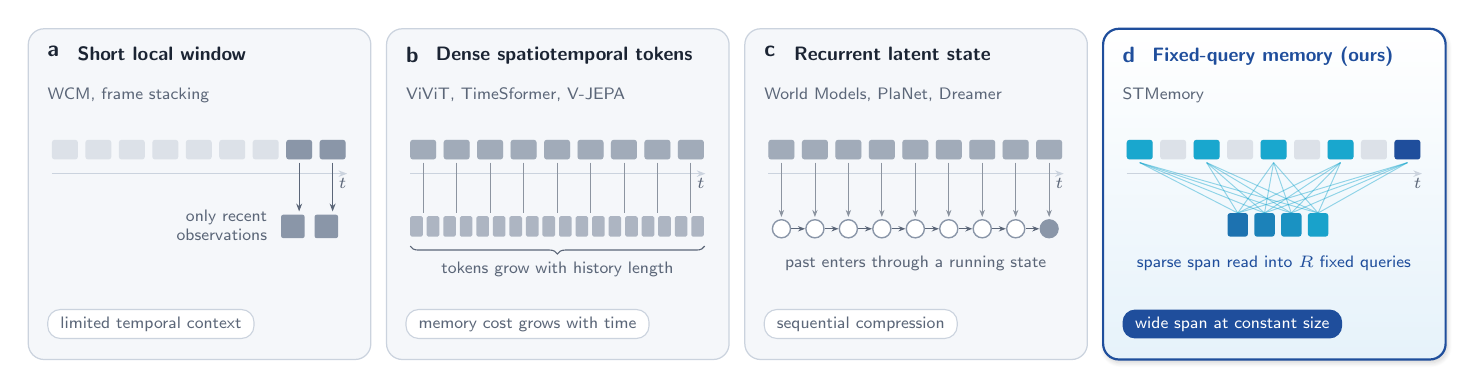
\begin{tikzpicture}[x=1mm,y=1mm]

% ---------------------------------------------------------------- a short window
\draw[card] (0,0) rectangle (43.5,42);
\node[let] at (2.4,39.8) {a};
\node[ttl] at (6.2,39.8) {Short local window};
\strip{3}
\foreach \i in {7,8}{\fill[fr, slate] ($(3,25.4)+(\i*4.25,0)$) rectangle ++(3.3,2.5);}
\foreach \i in {7,8}{\draw[sub, line width=.4pt, -{Stealth[length=1mm]}] ($(3,25.0)+(\i*4.25+1.65,0)$) -- ++(0,-6.2);}
\foreach \j in {0,1}{\fill[slate, rounded corners=.3mm] ($(32.1,15.4)+(\j*4.25,0)$) rectangle ++(3.0,3.0);}
\node[lbl, anchor=east, align=right] at (30.4,17) {only recent\\observations};
\node[chip, fill=white, draw=rule, text=sub, anchor=south west] at (2.4,2.6) {limited temporal context};
\node[lbl, anchor=north west] at (2.4,34.6) {WCM, frame stacking};

% ---------------------------------------------------------------- b dense tokens
\begin{scope}[xshift=45.5mm]
\draw[card] (0,0) rectangle (43.5,42);
\node[let] at (2.4,39.8) {b};
\node[ttl] at (6.2,39.8) {Dense spatiotemporal tokens};
\strip{3}
\foreach \i in {0,...,8}{\fill[fr, slate!80] ($(3,25.4)+(\i*4.25,0)$) rectangle ++(3.3,2.5);}
\foreach \j in {0,...,17}{\fill[slate!70, rounded corners=.2mm] ($(3,15.6)+(\j*2.1,0)$) rectangle ++(1.6,2.6);}
\foreach \i in {0,...,8}{\draw[sub!70, line width=.3pt] ($(3,25.0)+(\i*4.25+1.65,0)$) -- ($(3,18.6)+(\i*4.25+1.65,0)$);}
\draw[decorate, decoration={brace, mirror, amplitude=1mm}, sub, line width=.4pt] (3,14.4) -- (40.4,14.4);
\node[lbl, anchor=north] at (21.7,12.4) {tokens grow with history length};
\node[chip, fill=white, draw=rule, text=sub, anchor=south west] at (2.4,2.6) {memory cost grows with time};
\node[lbl, anchor=north west] at (2.4,34.6) {ViViT, TimeSformer, V-JEPA};
\end{scope}

% ---------------------------------------------------------------- c recurrent state
\begin{scope}[xshift=91mm]
\draw[card] (0,0) rectangle (43.5,42);
\node[let] at (2.4,39.8) {c};
\node[ttl] at (6.2,39.8) {Recurrent latent state};
\strip{3}
\foreach \i in {0,...,8}{\fill[fr, slate!80] ($(3,25.4)+(\i*4.25,0)$) rectangle ++(3.3,2.5);}
\foreach \i in {0,...,8}{
  \coordinate (h\i) at ($(3,16.6)+(\i*4.25+1.65,0)$);
  \draw[sub!70, line width=.3pt, -{Stealth[length=.9mm]}] ($(3,25.0)+(\i*4.25+1.65,0)$) -- ($(h\i)+(0,1.5)$);
}
\foreach \i [evaluate=\i as \j using int(\i+1)] in {0,...,7}{\draw[sub, line width=.4pt, -{Stealth[length=.9mm]}] ($(h\i)+(1.25,0)$) -- ($(h\j)+(-1.25,0)$);}
\foreach \i in {0,...,7}{\fill[white, draw=slate, line width=.5pt] (h\i) circle (1.15mm);}
\fill[slate, draw=slate] (h8) circle (1.15mm);
\node[lbl, anchor=north] at (21.7,13.2) {past enters through a running state};
\node[chip, fill=white, draw=rule, text=sub, anchor=south west] at (2.4,2.6) {sequential compression};
\node[lbl, anchor=north west] at (2.4,34.6) {World Models, PlaNet, Dreamer};
\end{scope}

% ---------------------------------------------------------------- d ours
\begin{scope}[xshift=136.5mm]
\draw[ours] (0,0) rectangle (43.5,42);
\node[let, text=cobalt] at (2.4,39.8) {d};
\node[ttl, text=cobalt] at (6.2,39.8) {Fixed-query memory (ours)};
\strip{3}
\foreach \i/\c in {0/cyan,2/cyan,4/cyan,6/cyan,8/cobalt}{\fill[fr, \c] ($(3,25.4)+(\i*4.25,0)$) rectangle ++(3.3,2.5);}
\foreach \i in {0,2,4,6,8}{
  \foreach \j in {0,...,3}{
    \draw[cyan, opacity=.45, line width=.35pt] ($(3,25.0)+(\i*4.25+1.65,0)$) -- ($(15.8,18.6)+(\j*3.4+1.3,0)$);
  }
}
\foreach \j in {0,...,3}{
  \pgfmathtruncatemacro{\m}{40+\j*18}
  \fill[cyan!\m!cobalt, rounded corners=.35mm] ($(15.8,15.6)+(\j*3.4,0)$) rectangle ++(2.6,3.0);
}
\node[lbl, anchor=north, text=cobalt] at (21.7,13.2) {sparse span read into $R$ fixed queries};
\node[chip, fill=cobalt, text=white, anchor=south west] at (2.4,2.6) {wide span at constant size};
\node[lbl, anchor=north west] at (2.4,34.6) {STMemory};
\end{scope}
\end{tikzpicture}
\end{document}
